\documentclass[10pt,letterpaper]{article}
\usepackage[margin=0.7in]{geometry}
\usepackage[T1]{fontenc}
\usepackage[utf8]{inputenc}
\usepackage{hyperref}
\usepackage{xcolor}
\usepackage{longtable}
\usepackage{array}
\usepackage{enumitem}
\usepackage{fvextra}
\usepackage{float}
\usepackage{graphicx}
\usepackage{tikz}
\usetikzlibrary{arrows.meta,positioning}
\setlist{nosep,leftmargin=*}
\hypersetup{colorlinks=true,linkcolor=blue,urlcolor=blue}
\DefineVerbatimEnvironment{Verbatim}{Verbatim}{fontsize=\scriptsize,breaklines=true,breakanywhere=true}
\title{
\includegraphics[width=0.24\textwidth]{assets/logo-red-neuronal-utm.png}\\[1em]Sabia: AI Research Insights\\Technical Report for the REST API and Integrated GUI}
\author{Ignacio Arroyo Fern\'andez\\Universidad Tecnol\'ogica de la Mixteca (UTM)\\\texttt{iaf [at] gs [dot] utm [dot] mx}\and Eduardo Varela Hern\'andez\\LaSalle Oaxaca\and Luis Felipe Morales\\LaSalle Oaxaca\\[0.75em]Secihti Ciencia de Frontera Grant CF-2023-I-2854}
\date{2026-04-25}
\begin{document}
\maketitle
\tableofcontents
\newpage

\textbf{Technical Report for the REST API and Integrated GUI}

Project context: academic research project funded by \textbf{Secihti Ciencia de Frontera, Grant CF-2023-I-2854}.

Source inspected: \texttt{blue-demon:/home/iarroyof/sabia/ai-research-insights}

GitHub repository: \url{https://github.com/iarroyof/ai-research-insights}

Verified commit: \texttt{54029058dc360cf000e053d08f6d49979c3bcd63}

Report date: \texttt{2026-04-25}

\section{Executive Summary}

Sabia: AI Research Insights is a containerized biomedical research platform for searching scientific evidence, selecting relevant sentences/triplets, generating context-grounded summaries and chat answers, and visualizing extracted biomedical knowledge as an interactive graph. The system combines a Streamlit GUI, a FastAPI REST API, tenant-aware middleware, hybrid search, object storage, relational annotation storage, graph storage, GPU-backed LLM inference, relation extraction, and background workers.

The current deployed API surface is defined by \texttt{services/api/app/main.py}. It mounts the \texttt{search}, \texttt{chat}, \texttt{triplets}, \texttt{papers}, \texttt{annotations}, and CSV ingest routers. Several additional router files exist in the repository but are not mounted; they are documented separately because source presence alone does not make them reachable through the running FastAPI app. The dataset and lung-cancer knowledge-base construction context is aligned with the scalable lung cancer knowledge-base work reported by Mart\'inez Cisneros et al. (2025), while the semantic reasoning and attention-based modeling context is aligned with Balderas-Mart\'inez et al. (2025).

\section{1. Project Overview and Architecture}

\subsection{Core Problem}

Biomedical literature review requires repeated movement between papers, snippets, relation extraction output, and expert interpretation. The project addresses this by combining:

\begin{itemize}
\item search over indexed scientific sentences and extracted triplets;
\item user selection of relevant evidence;
\item LLM-assisted chat and conditioned summarization grounded in selected context;
\item entity/relation triplet extraction and filtering;
\item interactive knowledge graph exploration;
\item annotation capture for later review, curation, or model-improvement workflows.
\end{itemize}

The software is not just a search UI. It is an evidence workbench where the REST API exposes the retrieval, ingestion, summarization, graph, and annotation capabilities, while the GUI orchestrates those capabilities into a researcher-facing workflow. Its data and knowledge-base workflow should be read as an implementation-oriented continuation of scalable biomedical knowledge-base construction methods for lung cancer literature (Mart\'inez Cisneros et al., 2025).

\subsection{Logical Architecture}


\begin{figure}[H]
\centering
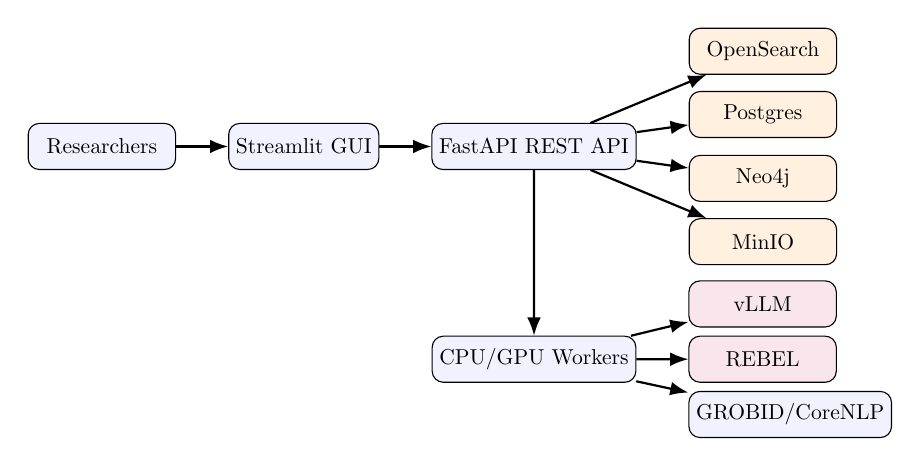
\begin{tikzpicture}[scale=0.78, every node/.style={transform shape}, node distance=0.65cm and 0.85cm, box/.style={draw, rounded corners, align=center, minimum width=2.4cm, minimum height=0.75cm, fill=blue!5}, store/.style={box,fill=orange!12}, gpu/.style={box,fill=purple!10}, arr/.style={-Latex,thick}]
\node[box] (u) {Researchers};
\node[box,right=of u] (ui) {Streamlit GUI};
\node[box,right=of ui] (api) {FastAPI REST API};
\node[store,right=of api,yshift=1.55cm] (os) {OpenSearch};
\node[store,right=of api,yshift=0.52cm] (pg) {Postgres};
\node[store,right=of api,yshift=-0.52cm] (neo) {Neo4j};
\node[store,right=of api,yshift=-1.55cm] (minio) {MinIO};
\node[box,below=2.70cm of api] (w) {CPU/GPU Workers};
\node[gpu,right=of w,yshift=0.9cm] (llm) {vLLM};
\node[gpu,right=of w] (rebel) {REBEL};
\node[box,right=of w,yshift=-0.9cm] (grobid) {GROBID/CoreNLP};
\draw[arr] (u)--(ui);
\draw[arr] (ui)--(api);
\draw[arr] (api)--(os);
\draw[arr] (api)--(pg);
\draw[arr] (api)--(neo);
\draw[arr] (api)--(minio);
\draw[arr] (api)--(w);
\draw[arr] (w)--(llm);
\draw[arr] (w)--(rebel);
\draw[arr] (w)--(grobid);
\end{tikzpicture}
\caption{Logical architecture of the Sabia platform.}
\end{figure}


Mermaid source: \href{docs/diagrams/logical-architecture.mmd}{docs/diagrams/logical-architecture.mmd}

\subsection{Physical Deployment Architecture}


\begin{figure}[H]
\centering
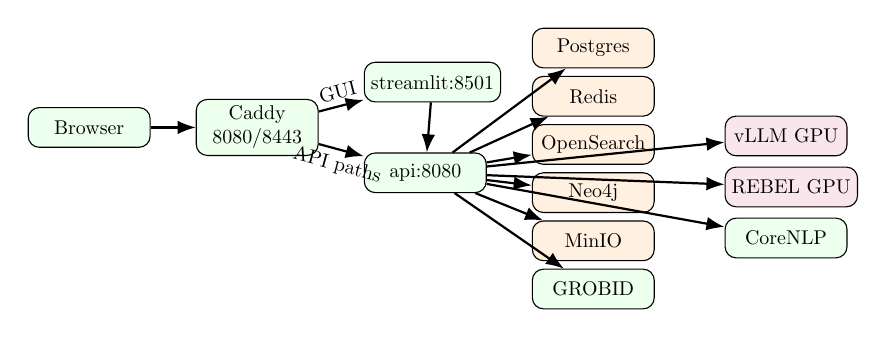
\begin{tikzpicture}[scale=0.72, every node/.style={transform shape}, node distance=0.65cm and 0.8cm, box/.style={draw, rounded corners, align=center, minimum width=2.15cm, minimum height=0.7cm, fill=green!7}, store/.style={box,fill=orange!12}, gpu/.style={box,fill=purple!10}, arr/.style={-Latex,thick}]
\node[box] (b) {Browser};
\node[box,right=of b] (caddy) {Caddy\\8080/8443};
\node[box,right=of caddy,yshift=0.8cm] (streamlit) {streamlit:8501};
\node[box,right=of caddy,yshift=-0.8cm] (api) {api:8080};
\node[store,right=of api,yshift=2.2cm] (pg) {Postgres};
\node[store,right=of api,yshift=1.35cm] (redis) {Redis};
\node[store,right=of api,yshift=0.5cm] (os) {OpenSearch};
\node[store,right=of api,yshift=-0.35cm] (neo) {Neo4j};
\node[store,right=of api,yshift=-1.2cm] (minio) {MinIO};
\node[box,right=of api,yshift=-2.05cm] (grobid) {GROBID};
\node[gpu,right=4.2cm of api,yshift=0.65cm] (llm) {vLLM GPU};
\node[gpu,right=4.2cm of api,yshift=-0.25cm] (rebel) {REBEL GPU};
\node[box,right=4.2cm of api,yshift=-1.15cm] (core) {CoreNLP};
\draw[arr] (b)--(caddy);
\draw[arr] (caddy)--node[above,sloped]{GUI}(streamlit);
\draw[arr] (caddy)--node[below,sloped]{API paths}(api);
\draw[arr] (streamlit)--(api);
\foreach \n in {pg,redis,os,neo,minio,grobid,llm,rebel,core}{\draw[arr] (api)--(\n);}
\end{tikzpicture}
\caption{Physical Docker Compose deployment and service communication.}
\end{figure}


Mermaid source: \href{docs/diagrams/physical-deployment.mmd}{docs/diagrams/physical-deployment.mmd}

\subsection{Main Runtime Components}

\begin{itemize}
\item \textbf{Caddy} listens on ports \texttt{8080} and \texttt{8443}. It reverse-proxies API paths such as \texttt{/search*}, \texttt{/chat*}, \texttt{/papers*}, \texttt{/triplets*}, \texttt{/annotations*}, and \texttt{/health} to the FastAPI service. All other paths are routed to Streamlit.
\item \textbf{FastAPI API} runs \texttt{uvicorn app.main:app --host 0.0.0.0 --port 8080} and exposes the REST API.
\item \textbf{Streamlit GUI} provides the researcher workflow and calls the API using \texttt{httpx}.
\item \textbf{Postgres} stores relational application data such as annotations and uses a tenant context intended for RLS policies.
\item \textbf{OpenSearch} stores searchable sentence/triplet indexes and supports hybrid lexical/vector retrieval.
\item \textbf{Neo4j} stores graph representations for entities and relations.
\item \textbf{MinIO} stores uploaded PDF/TXT objects.
\item \textbf{Redis/Celery workers} support asynchronous ingestion and processing work.
\item \textbf{GROBID} extracts structured metadata from scientific PDFs.
\item \textbf{vLLM} serves an OpenAI-compatible local LLM endpoint using \texttt{HuggingFaceH4/zephyr-7b-beta}.
\item \textbf{REBEL} is the primary relation extraction service. CoreNLP/OpenIE is configured as a fallback path.
\end{itemize}

\subsection{Technology Stack}

\begin{scriptsize}
\begin{longtable}{>{\raggedright\arraybackslash}p{3.35in}>{\raggedright\arraybackslash}p{3.35in}}
Layer & Technologies Observed \\
\hline
API framework & Python, FastAPI \texttt{0.112.0}, Uvicorn \texttt{0.30.5}, Pydantic \texttt{2.8.2}, Pydantic Settings \\
GUI & Streamlit \texttt{1.38.0}, \texttt{httpx}, Streamlit session state, Streamlit secrets \\
Search & OpenSearch \texttt{2.13.0}, BM25/vector hybrid settings, sentence-transformers optional embeddings \\
Data storage & Postgres \texttt{16}, MinIO, Neo4j \texttt{5.23.0-community}, Redis \\
Background processing & Celery \texttt{5.4.0}, CPU/GPU worker containers \\
NLP/AI & vLLM OpenAI-compatible server, Zephyr 7B, REBEL, Stanford CoreNLP, GROBID, transformers, torch, spaCy/scispaCy \\
Proxy/deployment & Docker Compose, Caddy, NVIDIA runtime for GPU containers \\
API documentation style & FastAPI/OpenAPI-ready route definitions, supplemented here by source-derived technical documentation \\
\end{longtable}
\end{scriptsize}

The semantic modeling layer combines indexed triplets, vector search, entity/relation representations, and context-conditioned LLM prompting. This design is consistent with prior work on semantic reasoning with standard attention-based models in chronic disease literature, where attention-based representations are used to support semantic inference over biomedical text (Balderas-Mart\'inez et al., 2025).

\section{2. REST API Specification}

\subsection{Base URLs}

\begin{itemize}
\item Internal Docker network API URL: \texttt{\url{http://api:8080}}
\item Host-published API URL in Compose: \texttt{\url{http://localhost:18081}}
\item Caddy public API paths: \texttt{\url{http://localhost:8080/<api-path>}}
\item Streamlit public path: \texttt{\url{http://localhost:8080/}} through Caddy fallback routing
\end{itemize}

\subsection{Required Headers}

\begin{scriptsize}
\begin{longtable}{>{\raggedright\arraybackslash}p{2.23in}>{\raggedright\arraybackslash}p{2.23in}>{\raggedright\arraybackslash}p{2.23in}}
Header & Required & Purpose \\
\hline
\texttt{X-API-Key} & Required for all non-public endpoints & Compared against \texttt{API\_KEY} environment variable or \texttt{security.api\_key} from config. \\
\texttt{X-Tenant-Id} & Required for all normal endpoints except \texttt{/health}; optional/query fallback for \texttt{/triplets/graph/view} & Sets \texttt{request.state.tenant\_id}; used by storage/search/annotation operations. \\
\texttt{Content-Type: application/json} & Required for JSON POST/PUT requests & Tells FastAPI to parse JSON bodies. \\
\texttt{x-user-id} & Optional for annotation endpoints & Stored as annotation \texttt{user\_id} when provided. \\
\end{longtable}
\end{scriptsize}

Public paths in current middleware: \texttt{/health} and \texttt{/triplets/graph/view*}.

\subsection{Deployed Endpoint Inventory}

\begin{scriptsize}
\begin{longtable}{>{\raggedright\arraybackslash}p{1.34in}>{\raggedright\arraybackslash}p{1.34in}>{\raggedright\arraybackslash}p{1.34in}>{\raggedright\arraybackslash}p{1.34in}>{\raggedright\arraybackslash}p{1.34in}}
Method & URI & Tag & Auth & Purpose \\
\hline
GET & /health & Health & Public & Returns \{'status':'ok'\}. \\
POST & /search/ & Search & API key + tenant & Hybrid search over papers/triplets/chats target model. Returns items alias for hits. \\
POST & /chat/ & Chat & API key + tenant & Streams server-sent events with token, citations, and final messages. \\
POST & /papers/upload & Papers & API key + tenant & Multipart PDF/TXT upload to MinIO; enqueues URI ingestion when task helper is wired. \\
POST & /papers/link & Papers & API key + tenant & Accepts article/direct links and enqueues link ingestion when task helper is wired. \\
POST & /papers/ncbi & Papers & API key + tenant & Accepts PMID list and enqueues NCBI ingestion when task helper is wired. \\
POST & /papers/summarize\_conditioned & Papers & API key + tenant & RAG/LLM summary over selected items; returns paragraphs and support sentences. \\
POST & /triplets/csv & Triplets & API key + tenant & Uploads CSV triplets; validates entity probabilities and confidence thresholds. \\
POST & /triplets/ingest\_csv & Triplets & API key + tenant & Uploads CSV through ingest\_csv\_triplets helper. \\
POST & /triplets/suggest & Triplets & API key + tenant & Runs relation extraction on supplied sentences. \\
POST & /triplets/graph/build & Triplets & API key + tenant & Builds graph candidate triple IDs from selected sentences. \\
GET & /triplets/graph & Triplets & API key + tenant & Returns graph JSON for comma-separated triple IDs. \\
GET & /triplets/graph/view & Graph & Public API key bypass; tenant header/query & Returns browser-friendly vis-network HTML graph viewer. \\
GET & /triplets/search & Triplets & API key + tenant & Searches triplet index by q, confidence\_min, entity\_type, and pmid. \\
POST & /triplets/classify & Classification & API key + tenant & Classifies entities with the NER/zero-shot classifier. \\
POST & /triplets/sync & Sync & API key + tenant & Manually syncs OpenSearch triplets into Neo4j. \\
POST & /annotations & Annotations & API key + tenant & Creates one annotation with optional idempotency key. \\
POST & /annotations/batch & Annotations & API key + tenant & Creates up to 500 annotations. \\
GET & /annotations & Annotations & API key + tenant & Lists annotations with filters and cursor pagination. \\
PUT & /annotations/\{annotation\_id\} & Annotations & API key + tenant & Updates kind, payload, page, or bbox. \\
DELETE & /annotations/\{annotation\_id\} & Annotations & API key + tenant & Deletes annotation for current tenant. \\
GET & /annotations/export & Annotations & API key + tenant & Streams NDJSON annotations for downstream training/RLHF workflows. \\
\end{longtable}
\end{scriptsize}

\subsection{Source Routers Not Currently Mounted}

These files exist under \texttt{services/api/app/routers}, but \texttt{services/api/app/main.py} does not include them with \texttt{app.include\_router(...)}.

\begin{scriptsize}
\begin{longtable}{>{\raggedright\arraybackslash}p{1.68in}>{\raggedright\arraybackslash}p{1.68in}>{\raggedright\arraybackslash}p{1.68in}>{\raggedright\arraybackslash}p{1.68in}}
Method & URI & Source & Status \\
\hline
POST & /chat/history/search & chat\_history.py & Defined as POST but not mounted; Streamlit currently calls GET, so the GUI history search will not work unless mounted and aligned. \\
GET & /chat/session/\{session\_id\}/messages & chat\_sessions.py & Defined but not mounted. \\
POST & /export/triples.csv & export.py & Defined but not mounted. \\
POST & /jobs/backfill/probabilities & jobs.py & Defined but not mounted. \\
POST & /predict/probabilities & probabilities.py & Defined but not mounted. \\
\end{longtable}
\end{scriptsize}

\subsection{Request and Response Models}

\begin{scriptsize}
\begin{longtable}{>{\raggedright\arraybackslash}p{3.35in}>{\raggedright\arraybackslash}p{3.35in}}
Model & Fields \\
\hline
SearchRequest & \texttt{query: str}, \texttt{target: papers|triplets|chats|all = all}, \texttt{filters: object = \{\}}, \texttt{k: 1..200 = 20} \\
SearchResponse/SearchHit & \texttt{items}: list of hits with \texttt{paper\_id}, \texttt{title}, \texttt{pmid}, \texttt{pmcid}, \texttt{page}, \texttt{sent\_id}, \texttt{score}, \texttt{text}, \texttt{subject}, \texttt{relation}, \texttt{object}, \texttt{confidence}. \\
ChatRequest & \texttt{message: str}, \texttt{items: ChatItem[]}, \texttt{session\_id?: str}, \texttt{options: \{allow\_extra\_retrieval, token\_budget, confidence\_min\}}. \\
ConditionedSummaryRequest & \texttt{message: str}, \texttt{items: ConditionedSummaryItem[]}, \texttt{options: object}. \\
ConditionedSummaryResponse & \texttt{paragraphs}: list of \texttt{\{text, support[]\}} where support carries sentence provenance and SVO fields. \\
UploadResponse & \texttt{job\_id}, \texttt{num\_files}, \texttt{objects} stored as \texttt{s3://bucket/tenant/uploads/...}. \\
AnnotationCreate & \texttt{paper\_id}, \texttt{sent\_id?}, \texttt{kind: highlight|note|like|unlike}, \texttt{payload}, \texttt{page?}, \texttt{bbox?}, \texttt{idempotency\_key?}. \\
AnnotationOut & \texttt{id}, \texttt{paper\_id}, \texttt{sent\_id}, \texttt{kind}, \texttt{payload}, \texttt{page}, \texttt{bbox}, \texttt{user\_id}, \texttt{created\_at}. \\
Triplet graph build response & \texttt{triple\_ids}, \texttt{count}, and \texttt{debug} metadata with selected item count, paper IDs, query terms, thresholds, and top\_k. \\
Classify response & \texttt{results} from NER classifier and \texttt{models\_available}. \\
\end{longtable}
\end{scriptsize}


\subsection{Request and response examples}

\subsubsection{Health}

\begin{Verbatim}[fontsize=\scriptsize,breaklines=true,breakanywhere=true]
curl http://localhost:8080/health
\end{Verbatim}

\begin{Verbatim}[fontsize=\scriptsize,breaklines=true,breakanywhere=true]
{"status": "ok"}
\end{Verbatim}

\subsubsection{Search}

\begin{Verbatim}[fontsize=\scriptsize,breaklines=true,breakanywhere=true]
curl -X POST http://localhost:8080/search/ \
  -H "X-API-Key: $API_KEY" \
  -H "X-Tenant-Id: default" \
  -H "Content-Type: application/json" \
  -d '{"query":"immunotherapy lung carcinoma","target":"all","filters":{"confidence_min":0.6},"k":3}'
\end{Verbatim}

\begin{Verbatim}[fontsize=\scriptsize,breaklines=true,breakanywhere=true]
{
  "items": [
    {
      "paper_id": "PMC123456.txt",
      "pmid": "12345678",
      "pmcid": "PMC123456",
      "sent_id": "sent-0001",
      "score": 12.84,
      "text": "PD-1 blockade improved response in lung carcinoma cohorts.",
      "subject": "PD-1 blockade",
      "relation": "improved",
      "object": "response",
      "confidence": 0.87
    }
  ]
}
\end{Verbatim}

Common errors:

\begin{Verbatim}[fontsize=\scriptsize,breaklines=true,breakanywhere=true]
{"detail": "Invalid X-API-Key"}
\end{Verbatim}

\begin{Verbatim}[fontsize=\scriptsize,breaklines=true,breakanywhere=true]
{"detail": "Search failed: RuntimeError: <backend message>"}
\end{Verbatim}

\subsubsection{Chat with pinned context}

The chat endpoint returns \texttt{text/event-stream}; clients should parse each \texttt{data:} line as JSON.

\begin{Verbatim}[fontsize=\scriptsize,breaklines=true,breakanywhere=true]
curl -N -X POST http://localhost:8080/chat/ \
  -H "X-API-Key: $API_KEY" \
  -H "X-Tenant-Id: default" \
  -H "Content-Type: application/json" \
  -d '{"message":"Summarize the evidence.","items":[{"paper_id":"PMC123456.txt","sent_id":"sent-0001","text":"PD-1 blockade improved response."}],"options":{"allow_extra_retrieval":false}}'
\end{Verbatim}

\begin{Verbatim}[fontsize=\scriptsize,breaklines=true,breakanywhere=true]
data: {"type":"token","data":"PD-1 blockade..."}
data: {"type":"citations","data":{"snippets":[{"paper_id":"PMC123456.txt","sent_id":"sent-0001"}]}}
data: {"type":"final","data":{"done":true,"session_id":"6fd7e1d1-1c9b-4b5d-9a10-8ac5e9f27e33"}}
\end{Verbatim}

\subsubsection{Upload papers}

\begin{Verbatim}[fontsize=\scriptsize,breaklines=true,breakanywhere=true]
curl -X POST http://localhost:8080/papers/upload \
  -H "X-API-Key: $API_KEY" \
  -H "X-Tenant-Id: default" \
  -F "files=@article.pdf"
\end{Verbatim}

\begin{Verbatim}[fontsize=\scriptsize,breaklines=true,breakanywhere=true]
{
  "job_id": "8a6e0f31-7e8a-4e83-b39e-bb971c2b0793",
  "num_files": 1,
  "objects": ["s3://papers/default/uploads/uuid_article.pdf"]
}
\end{Verbatim}

If the ingestion task helper is not wired:

\begin{Verbatim}[fontsize=\scriptsize,breaklines=true,breakanywhere=true]
{"detail": "Ingestion task not wired. Implement app.tasks.ingest.enqueue_ingest_uris(tenant, uris) to process uploaded objects."}
\end{Verbatim}

\subsubsection{Link and PMID ingestion}

\begin{Verbatim}[fontsize=\scriptsize,breaklines=true,breakanywhere=true]
[
  {"url": "https://pubmed.ncbi.nlm.nih.gov/12345678/", "metadata": {"topic": "immunotherapy"}}
]
\end{Verbatim}

\begin{Verbatim}[fontsize=\scriptsize,breaklines=true,breakanywhere=true]
{"job_id": "link-job-id", "num_links": 1}
\end{Verbatim}

\begin{Verbatim}[fontsize=\scriptsize,breaklines=true,breakanywhere=true]
{"pmids": ["12345678", "23456789"]}
\end{Verbatim}

\begin{Verbatim}[fontsize=\scriptsize,breaklines=true,breakanywhere=true]
{"job_id": "pmid-job-id", "num_pmids": 2}
\end{Verbatim}

\subsubsection{Conditioned summary}

\begin{Verbatim}[fontsize=\scriptsize,breaklines=true,breakanywhere=true]
{
  "message": "What are the main immunotherapy strategies for lung carcinoma?",
  "items": [
    {
      "paper_id": "PMC123456.txt",
      "sent_id": "sent-0001",
      "text": "PD-1 blockade improved response in lung carcinoma.",
      "subject": "PD-1 blockade",
      "relation": "improved",
      "object": "response"
    }
  ],
  "options": {"max_paragraphs": 3, "confidence_min": 0.5}
}
\end{Verbatim}

\begin{Verbatim}[fontsize=\scriptsize,breaklines=true,breakanywhere=true]
{
  "paragraphs": [
    {
      "text": "The selected evidence emphasizes immune checkpoint inhibition...",
      "support": [
        {
          "paper_id": "PMC123456.txt",
          "sent_id": "sent-0001",
          "text": "PD-1 blockade improved response in lung carcinoma.",
          "subject": "PD-1 blockade",
          "predicate": "improved",
          "object": "response",
          "pmid": "12345678",
          "pmcid": "PMC123456",
          "page": 4
        }
      ]
    }
  ]
}
\end{Verbatim}

\subsubsection{CSV triplet upload}

\begin{Verbatim}[fontsize=\scriptsize,breaklines=true,breakanywhere=true]
curl -X POST http://localhost:8080/triplets/csv \
  -H "X-API-Key: $API_KEY" \
  -H "X-Tenant-Id: default" \
  -F "file=@triplets.csv"
\end{Verbatim}

\begin{Verbatim}[fontsize=\scriptsize,breaklines=true,breakanywhere=true]
{"accepted": 1200, "filtered": 83, "job_id": "csv:6c4f8040-7b33-4cf8-b7a4-d7143b646736"}
\end{Verbatim}

Error:

\begin{Verbatim}[fontsize=\scriptsize,breaklines=true,breakanywhere=true]
{"detail": "Invalid file type (expected .csv)"}
\end{Verbatim}

\subsubsection{Suggest triplets}

\begin{Verbatim}[fontsize=\scriptsize,breaklines=true,breakanywhere=true]
[
  "Pembrolizumab targets PD-1 in lung cancer therapy."
]
\end{Verbatim}

\begin{Verbatim}[fontsize=\scriptsize,breaklines=true,breakanywhere=true]
[
  {
    "subject": "Pembrolizumab",
    "predicate": "targets",
    "object": "PD-1",
    "confidence": 0.81
  }
]
\end{Verbatim}

\subsubsection{Build graph from selected rows}

\begin{Verbatim}[fontsize=\scriptsize,breaklines=true,breakanywhere=true]
curl -X POST "http://localhost:8080/triplets/graph/build?confidence_min=0.6&ebio_min=0.3&top_k=50" \
  -H "X-API-Key: $API_KEY" \
  -H "X-Tenant-Id: default" \
  -H "Content-Type: application/json" \
  -d '[{"paper_id":"PMC123456.txt","sent_id":"sent-0001","text":"PD-1 blockade improved response."}]'
\end{Verbatim}

\begin{Verbatim}[fontsize=\scriptsize,breaklines=true,breakanywhere=true]
{
  "triple_ids": ["triplet-1", "triplet-2"],
  "count": 2,
  "debug": {
    "mode": "semantic_search_filtered",
    "items_in": 1,
    "paper_ids": ["PMC123456.txt"],
    "query_terms": "PD-1 blockade improved response",
    "triples_found": 2,
    "confidence_min": 0.6,
    "ebio_min": 0.3,
    "top_k": 50
  }
}
\end{Verbatim}

\subsubsection{Graph JSON and viewer}

\begin{Verbatim}[fontsize=\scriptsize,breaklines=true,breakanywhere=true]
curl "http://localhost:8080/triplets/graph?triple_ids=triplet-1,triplet-2&confidence_min=0.6" \
  -H "X-API-Key: $API_KEY" \
  -H "X-Tenant-Id: default"
\end{Verbatim}

\begin{Verbatim}[fontsize=\scriptsize,breaklines=true,breakanywhere=true]
{
  "nodes": [{"id": "PD-1", "label": "PD-1", "type": "protein"}],
  "edges": [{"id": "triplet-1", "source": "Pembrolizumab", "target": "PD-1", "label": "targets", "confidence": 0.81}]
}
\end{Verbatim}

The HTML viewer is browser-facing and accepts the API key bypass in middleware:

\begin{Verbatim}[fontsize=\scriptsize,breaklines=true,breakanywhere=true]
http://localhost:8080/triplets/graph/view?triple_ids=triplet-1,triplet-2&confidence_min=0.6&tenant=default
\end{Verbatim}

\subsubsection{Annotation CRUD}

\begin{Verbatim}[fontsize=\scriptsize,breaklines=true,breakanywhere=true]
{
  "paper_id": "PMC123456.txt",
  "sent_id": "sent-0001",
  "kind": "note",
  "payload": {"text": "Strong evidence for checkpoint inhibition."},
  "page": 4,
  "bbox": {"x": 100, "y": 220, "width": 250, "height": 40},
  "idempotency_key": "client-generated-key"
}
\end{Verbatim}

\begin{Verbatim}[fontsize=\scriptsize,breaklines=true,breakanywhere=true]
{
  "id": "9df9f20c-6dd4-4e6d-aacf-4bbf8eab8b24",
  "paper_id": "PMC123456.txt",
  "sent_id": "sent-0001",
  "kind": "note",
  "payload": {"text": "Strong evidence for checkpoint inhibition."},
  "page": 4,
  "bbox": {"x": 100, "y": 220, "width": 250, "height": 40},
  "user_id": "researcher-1",
  "created_at": "2026-04-24T12:00:00Z"
}
\end{Verbatim}

List response:

\begin{Verbatim}[fontsize=\scriptsize,breaklines=true,breakanywhere=true]
{"items": [{"id": "9df9f20c-6dd4-4e6d-aacf-4bbf8eab8b24", "paper_id": "PMC123456.txt", "sent_id": "sent-0001", "kind": "note", "payload": {}, "page": 4, "bbox": null, "user_id": null, "created_at": "2026-04-24T12:00:00Z"}], "next_cursor": null}
\end{Verbatim}

Delete response:

\begin{Verbatim}[fontsize=\scriptsize,breaklines=true,breakanywhere=true]
{"status": "ok", "deleted": 1}
\end{Verbatim}

Common annotation errors:

\begin{Verbatim}[fontsize=\scriptsize,breaklines=true,breakanywhere=true]
{"detail": "Missing X-Tenant-Id"}
\end{Verbatim}

\begin{Verbatim}[fontsize=\scriptsize,breaklines=true,breakanywhere=true]
{"detail": "Annotation not found"}
\end{Verbatim}

\begin{Verbatim}[fontsize=\scriptsize,breaklines=true,breakanywhere=true]
{"detail": "Invalid cursor"}
\end{Verbatim}

\subsubsection{Entity classification}

\begin{Verbatim}[fontsize=\scriptsize,breaklines=true,breakanywhere=true]
{"entities": ["PD-1", "lung carcinoma", "immune checkpoint inhibitor"]}
\end{Verbatim}

\begin{Verbatim}[fontsize=\scriptsize,breaklines=true,breakanywhere=true]
{
  "results": [
    {"text": "PD-1", "entity_type": "biomedical", "scores": {"EBio": 0.91, "NGen": 0.06, "other": 0.03}}
  ],
  "models_available": ["facebook/bart-large-mnli"]
}
\end{Verbatim}

If models are unavailable:

\begin{Verbatim}[fontsize=\scriptsize,breaklines=true,breakanywhere=true]
{"detail": "NER models not loaded. Please install models first."}
\end{Verbatim}

\subsubsection{Manual Neo4j sync}

\begin{Verbatim}[fontsize=\scriptsize,breaklines=true,breakanywhere=true]
curl -X POST "http://localhost:8080/triplets/sync?max_triplets=5000" \
  -H "X-API-Key: $API_KEY" \
  -H "X-Tenant-Id: default"
\end{Verbatim}

\begin{Verbatim}[fontsize=\scriptsize,breaklines=true,breakanywhere=true]
{
  "status": "success",
  "tenant": "default",
  "index": "triplets_default",
  "stats": {"nodes": 1200, "relationships": 980}
}
\end{Verbatim}


\subsection{Authentication and Security}

Authentication is API-key based. The middleware accepts the key in either:

\begin{itemize}
\item \texttt{X-API-Key: <value>} header, which is the primary method;
\item \texttt{?api\_key=<value>} query parameter, which is a fallback for browser-only flows.
\end{itemize}

The expected key is resolved from \texttt{API\_KEY} first and then from \texttt{settings.security.api\_key}. If \texttt{security.require\_api\_key} is false, key checking is bypassed. The configuration file also contains \texttt{enable\_hmac} and \texttt{rate\_limit\_per\_min}, but the inspected middleware does not implement HMAC verification or rate limiting yet.

Tenant isolation is handled by \texttt{TenantMiddleware}, which requires \texttt{X-Tenant-Id} for normal endpoints and stores it as \texttt{request.state.tenant\_id}. The annotations router sets \texttt{app.tenant\_id} in Postgres using \texttt{set\_config(...)}, which is intended to align with row-level security policies.

Security implications:

\begin{itemize}
\item API keys are long-lived shared secrets; rotate them through \texttt{.env}/deployment secret management.
\item Do not expose non-public endpoints without HTTPS in production.
\item \texttt{/triplets/graph/view} is intentionally public in middleware; it should only expose non-sensitive graph IDs or be protected before external deployment.
\item Query-string API keys are convenient for browsers but can leak through logs and history; prefer headers where possible.
\item HMAC and rate limiting are configured but not enforced in the inspected middleware.
\end{itemize}

\subsection{Error Handling and Troubleshooting}

\begin{scriptsize}
\begin{longtable}{>{\raggedright\arraybackslash}p{1.68in}>{\raggedright\arraybackslash}p{1.68in}>{\raggedright\arraybackslash}p{1.68in}>{\raggedright\arraybackslash}p{1.68in}}
Code & Current Sources & Meaning & Troubleshooting \\
\hline
\texttt{400} & Tenant middleware, CSV upload, annotations, graph & Missing tenant, invalid cursor, invalid file type, empty update body, missing triple IDs/entities & Check \texttt{X-Tenant-Id}, query parameters, file extension, request body, and required IDs. \\
\texttt{403} & Security middleware & Missing or invalid API key & Confirm \texttt{X-API-Key} equals \texttt{API\_KEY} in the API container environment. \\
\texttt{404} & Annotation update/delete & Annotation not found for current tenant & Verify \texttt{annotation\_id} and tenant context. \\
\texttt{422} & FastAPI/Pydantic & Invalid schema, missing fields, invalid ranges/patterns & Check request body against the models above. \\
\texttt{500} & Search, annotations DB, Neo4j sync, graph viewer & Backend exception & Inspect API logs, upstream service availability, and tenant/index names. \\
\texttt{501} & Papers ingestion, triplet search & Optional helper/backend not wired & Implement the referenced task helper or enable the missing backend. \\
\texttt{502} & Paper upload to MinIO & Object storage failure & Check MinIO service, bucket, credentials, and network reachability. \\
\texttt{503} & Entity classifier & NER models not loaded & Install/load spaCy/scispaCy/zero-shot models and restart the API. \\
\end{longtable}
\end{scriptsize}

Recommended improvement: standardize error bodies into a stable shape such as \texttt{\{"error": \{"code": "...", "message": "...", "details": ...\}\}}, add request IDs, and document which errors are retryable.

\section{3. GUI and Integration Design}

\subsection{GUI User Journey}


\begin{figure}[H]
\centering
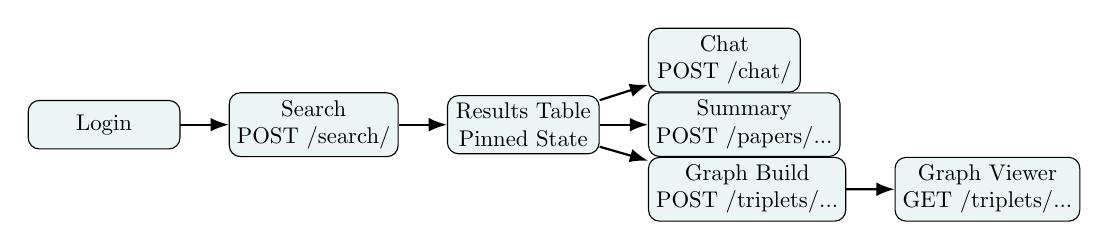
\begin{tikzpicture}[scale=0.82, every node/.style={transform shape}, node distance=0.75cm and 0.75cm, box/.style={draw, rounded corners, align=center, minimum width=2.35cm, minimum height=0.75cm, fill=teal!8}, arr/.style={-Latex,thick}]
\node[box] (login) {Login};
\node[box,right=of login] (search) {Search\\POST /search/};
\node[box,right=of search] (select) {Results Table\\Pinned State};
\node[box,right=of select,yshift=1.0cm] (chat) {Chat\\POST /chat/};
\node[box,right=of select] (summary) {Summary\\POST /papers/...};
\node[box,right=of select,yshift=-1.0cm] (graph) {Graph Build\\POST /triplets/...};
\node[box,right=of graph] (view) {Graph Viewer\\GET /triplets/...};
\draw[arr] (login)--(search);
\draw[arr] (search)--(select);
\draw[arr] (select)--(chat);
\draw[arr] (select)--(summary);
\draw[arr] (select)--(graph);
\draw[arr] (graph)--(view);
\end{tikzpicture}
\caption{GUI user journey and API interaction flow.}
\end{figure}


Mermaid source: \href{docs/diagrams/gui-api-flow.mmd}{docs/diagrams/gui-api-flow.mmd}

\subsection{Component and API Data Source Map}


\begin{figure}[H]
\centering
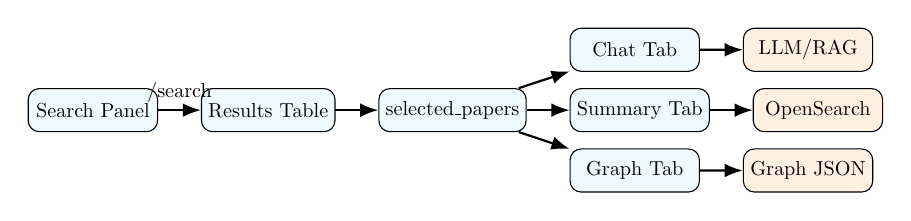
\begin{tikzpicture}[scale=0.73, every node/.style={transform shape}, node distance=0.75cm and 0.75cm, box/.style={draw, rounded corners, align=center, minimum width=2.25cm, minimum height=0.75cm, fill=cyan!7}, source/.style={box,fill=orange!12}, arr/.style={-Latex,thick}]
\node[box] (search) {Search Panel};
\node[box,right=of search] (results) {Results Table};
\node[box,right=of results] (state) {selected\_papers};
\node[box,right=of state,yshift=1.05cm] (chat) {Chat Tab};
\node[box,right=of state] (summary) {Summary Tab};
\node[box,right=of state,yshift=-1.05cm] (graph) {Graph Tab};
\node[source,right=of chat] (llm) {LLM/RAG};
\node[source,right=of summary] (os) {OpenSearch};
\node[source,right=of graph] (neo) {Graph JSON};
\draw[arr] (search)--node[above]{/search}(results);
\draw[arr] (results)--(state);
\draw[arr] (state)--(chat);
\draw[arr] (state)--(summary);
\draw[arr] (state)--(graph);
\draw[arr] (chat)--(llm);
\draw[arr] (summary)--(os);
\draw[arr] (graph)--(neo);
\end{tikzpicture}
\caption{GUI components and their backend data sources.}
\end{figure}


Mermaid source: \href{docs/diagrams/component-map.mmd}{docs/diagrams/component-map.mmd}

\subsection{Search-to-Graph Sequence}


\begin{figure}[H]
\centering
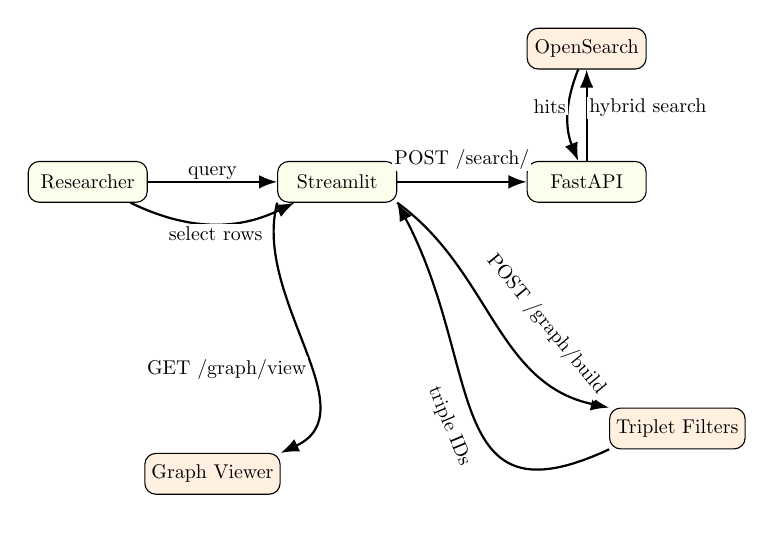
\begin{tikzpicture}[scale=0.72, every node/.style={transform shape}, box/.style={draw, rounded corners, align=center, minimum width=2.1cm, minimum height=0.72cm, fill=lime!8}, service/.style={box,fill=orange!12}, arr/.style={-Latex,thick}, lbl/.style={fill=white,inner sep=1pt}]
\node[box] (u) at (0,0) {Researcher};
\node[box] (gui) at (4.4,0) {Streamlit};
\node[box] (api) at (8.8,0) {FastAPI};
\node[service] (search) at (8.8,2.35) {OpenSearch};
\node[service] (filters) at (10.4,-4.35) {Triplet Filters};
\node[service] (viewer) at (2.2,-5.15) {Graph Viewer};
\draw[arr] (u)--node[lbl,above]{query}(gui);
\draw[arr] (gui)--node[lbl,above=5pt,pos=0.50]{POST /search/}(api);
\draw[arr] (api)--node[lbl,right,pos=0.58]{hybrid search}(search);
\draw[arr] (search) to[bend right=22] node[lbl,left,pos=0.40]{hits}(api);
\draw[arr] (u) to[bend right=26] node[lbl,below,pos=0.52]{select rows} (gui);
\draw[arr] (gui.south east) to[out=-36,in=168] node[lbl,above,sloped,pos=0.62,yshift=13pt]{POST /graph/build} (filters.north west);
\draw[arr] (filters.south west) to[out=205,in=-62,looseness=1.45] node[lbl,below,sloped,pos=0.50,yshift=-7pt]{triple IDs} (gui.south east);
\draw[arr] (gui.south west) to[out=-105,in=25] node[lbl,left,pos=0.58]{GET /graph/view} (viewer.north east);
\end{tikzpicture}
\caption{Search-to-graph sequence from query to interactive visualization.}
\end{figure}


\subsection{Main Screens and Intended Flow}

\begin{enumerate}
\item \textbf{Login screen}: Streamlit checks username/password against \texttt{st.secrets.passwords}. Successful login sets \texttt{st.session\_state["authenticated"] = True}.
\item \textbf{Search panel}: The user enters a biomedical query and Top K. The GUI sends \texttt{POST /search/} with \texttt{query}, \texttt{target}, \texttt{filters}, and \texttt{k}.
\item \textbf{Results table}: Results are sorted descending by \texttt{confidence}, displayed with subject/relation/object/text/provenance fields, and selected using checkbox cells in \texttt{st.data\_editor}.
\item \textbf{Pinned context state}: Selected rows are normalized into \texttt{st.session\_state["selected\_papers"]}.
\item \textbf{Chat tab}: The selected items are sent to \texttt{POST /chat/}. The GUI streams SSE tokens and later displays citations.
\item \textbf{Conditioned summary tab}: The selected items plus a question are sent to \texttt{POST /papers/summarize\_conditioned}.
\item \textbf{Triplets/Graph tab}: The selected items, confidence threshold, biomedical score threshold, and Top K are sent to \texttt{POST /triplets/graph/build}. The returned \texttt{triple\_ids} are stored in \texttt{st.session\_state["graph\_triple\_ids"]}.
\item \textbf{Graph viewer}: The GUI builds a URL for \texttt{GET /triplets/graph/view?triple\_ids=...\&confidence\_min=...\&tenant=...}, which returns a vis-network HTML graph.
\end{enumerate}

\subsection{API-UI Mapping}

\begin{scriptsize}
\begin{longtable}{>{\raggedright\arraybackslash}p{1.34in}>{\raggedright\arraybackslash}p{1.34in}>{\raggedright\arraybackslash}p{1.34in}>{\raggedright\arraybackslash}p{1.34in}>{\raggedright\arraybackslash}p{1.34in}}
UI Action & GUI State/Input & API Operation & API Output & GUI Effect \\
\hline
Login & \texttt{username}, \texttt{password} & No API call; Streamlit secrets check & Boolean auth state & Allows or stops app rendering. \\
Search & \texttt{q}, \texttt{k}, tenant, API key & \texttt{POST /search/} & \texttt{items} list & Populates \texttt{results}, clears previous selection. \\
Select rows & Edited data table & No API call & N/A & Updates \texttt{selected\_papers}. \\
Start Chat & \texttt{message}, selected items, \texttt{allow\_extra\_retrieval} & \texttt{POST /chat/} & SSE token/citations/final events & Streams answer and citations. \\
Run Conditioned Summary & \texttt{question}, selected items & \texttt{POST /papers/summarize\_conditioned} & \texttt{paragraphs} with support & Displays summary and supporting evidence. \\
Build graph & selected items, \texttt{confidence\_min}, \texttt{ebio\_min}, \texttt{top\_k} & \texttt{POST /triplets/graph/build} & \texttt{triple\_ids}, debug details & Stores graph IDs and shows debug metadata. \\
Open graph viewer & \texttt{graph\_triple\_ids}, tenant, confidence & \texttt{GET /triplets/graph/view} & HTML page & Opens interactive graph in a new tab. \\
Search history & \texttt{hist\_q} & Intended history search & Currently mismatched & GUI calls \texttt{GET /chat/history/search}, but source defines unmounted \texttt{POST /chat/history/search}. \\
\end{longtable}
\end{scriptsize}

\subsection{State Management}

The Streamlit GUI uses \texttt{st.session\_state} as its client-side state container:

\begin{itemize}
\item \texttt{authenticated}: login state.
\item \texttt{results}: latest search result set.
\item \texttt{selected\_papers}: normalized selected rows used by chat, summary, and graph workflows.
\item \texttt{history\_hits}: intended chat-history search result state.
\item \texttt{graph\_triple\_ids}: latest graph build output.
\end{itemize}

Sorting is performed client-side by confidence after search results arrive. Paging is not implemented in the GUI search result table; the API accepts \texttt{k}, and the Streamlit input limits it to 1-100. Filtering for graph construction is server-side through query parameters, while graph-view filtering is client-side inside the returned HTML page.

\subsection{Integration Finding}

The GUI contains a history-search feature, but it currently does not line up with the deployed API:

\begin{itemize}
\item GUI call: \texttt{GET /chat/history/search} with query parameters.
\item Source router: \texttt{POST /chat/history/search} with a \texttt{ChatSearchReq} JSON body.
\item Deployment: \texttt{chat\_history.py} is not mounted in \texttt{main.py}.
\end{itemize}

To make this feature operational, mount the router in \texttt{main.py} and either change the GUI to POST JSON or add a GET-compatible endpoint.

\section{4. Development and Maintenance}

\subsection{Setup and Installation}

Prerequisites:

\begin{itemize}
\item Docker and Docker Compose.
\item NVIDIA Container Toolkit for GPU services (\texttt{worker-gpu}, \texttt{llm}, \texttt{rebel-extractor}).
\item A \texttt{.env} file providing at least \texttt{API\_KEY}, \texttt{POSTGRES\_USER}, \texttt{POSTGRES\_PASSWORD}, \texttt{POSTGRES\_DB}, \texttt{NEO4J\_USER}, \texttt{NEO4J\_PASSWORD}, \texttt{MINIO\_ROOT\_USER}, \texttt{MINIO\_ROOT\_PASSWORD}, and \texttt{LLM\_MODEL\_ID} as needed.
\item Hugging Face model cache mounted at \texttt{/mnt/data/huggingface/hub} on the host, or an adjusted model volume path.
\end{itemize}

Typical startup:

\begin{Verbatim}[fontsize=\scriptsize,breaklines=true,breakanywhere=true]
cd /home/iarroyof/sabia/ai-research-insights
make build
make up
make ps
make logs
\end{Verbatim}

Manual Compose equivalent:

\begin{Verbatim}[fontsize=\scriptsize,breaklines=true,breakanywhere=true]
docker compose build
docker compose up -d
docker compose ps
docker compose logs -f api streamlit
\end{Verbatim}

Health check:

\begin{Verbatim}[fontsize=\scriptsize,breaklines=true,breakanywhere=true]
curl http://localhost:8080/health
\end{Verbatim}

Streamlit through Caddy:

\begin{Verbatim}[fontsize=\scriptsize,breaklines=true,breakanywhere=true]
http://localhost:8080/
\end{Verbatim}

Host-published API port from Compose:

\begin{Verbatim}[fontsize=\scriptsize,breaklines=true,breakanywhere=true]
http://localhost:18081/
\end{Verbatim}

OpenSearch host port:

\begin{Verbatim}[fontsize=\scriptsize,breaklines=true,breakanywhere=true]
http://localhost:19200/
\end{Verbatim}

Neo4j browser:

\begin{Verbatim}[fontsize=\scriptsize,breaklines=true,breakanywhere=true]
http://localhost:7474/
\end{Verbatim}

\subsection{Configuration}

The API reads \texttt{APP\_CONFIG=/app/config/default.yaml}, expands environment variables, and validates the config using Pydantic settings. Important sections:

\begin{itemize}
\item \texttt{security}: API key requirement, configured key, HMAC flag, configured rate limit.
\item \texttt{multi\_tenancy}: RLS strategy, default tenant, enforcement flag.
\item \texttt{postgres}: DSN assembled from environment variables.
\item \texttt{opensearch}: endpoint, vector dimension, BM25/vector retrieval settings, fusion weight.
\item \texttt{neo4j}: Bolt URI and credentials.
\item \texttt{minio}: object storage endpoint, credentials, bucket.
\item \texttt{llm}: OpenAI-compatible base URL, model, token limits, decoding parameters.
\item \texttt{re}: primary extractor and fallback extractor URLs.
\item \texttt{csv.thresholds}: biomedical and confidence thresholds used by CSV and graph workflows.
\item \texttt{classification}: zero-shot model and labels.
\end{itemize}

\subsection{Versioning Strategy}

The current FastAPI app declares version \texttt{0.1.0}, but the REST paths are not versioned by URI or header. Recommended strategy:

\begin{itemize}
\item Keep current paths stable as implicit \texttt{v1} until a breaking change is required.
\item Introduce \texttt{/v1/...} before external users depend on the API.
\item Add only backward-compatible response fields when possible.
\item For breaking schema changes, run \texttt{/v1} and \texttt{/v2} side by side through FastAPI router prefixes or Caddy routing.
\item Include \texttt{X-API-Version} or an explicit OpenAPI version in release notes for reproducibility.
\end{itemize}

\subsection{Observability}

Observed:

\begin{itemize}
\item Uvicorn/FastAPI runtime logging through Docker logs.
\item Caddy \texttt{log} directive enabled for public ingress.
\item \texttt{prometheus-client} is listed in API requirements, but no \texttt{/metrics} route was observed in mounted routers.
\item \texttt{monitor\_ingestion.sh} polls OpenSearch count/stats and tails API logs for ingestion progress.
\item \texttt{test\_partial\_data.sh} probes indexed triplet count and sample search behavior.
\end{itemize}

Recommended observability additions:

\begin{itemize}
\item Request ID middleware and \texttt{X-Request-ID} response header.
\item Structured JSON logs including method, path, status, latency, tenant, request ID, and upstream service timing.
\item Prometheus \texttt{/metrics} with request count, latency histogram, error count, queue depth, ingestion throughput, LLM latency, and extraction latency.
\item Health/readiness endpoints per dependency: Postgres, OpenSearch, Neo4j, MinIO, Redis, LLM, REBEL, GROBID.
\item Alerts for API 5xx rate, search latency, queue backlog, model container restarts, and disk usage in OpenSearch/MinIO/Neo4j volumes.
\end{itemize}

\subsection{Testing Report}

Observed test coverage is operational rather than unit-test based. The repository contains \texttt{test\_partial\_data.sh}, which verifies that the triplet index has enough documents and then sends sample search calls for \texttt{cancer} and \texttt{lung}. No pytest suite, integration test suite, or GUI usability test suite was found in the inspected tree.

Recommended test matrix:

\begin{scriptsize}
\begin{longtable}{>{\raggedright\arraybackslash}p{3.35in}>{\raggedright\arraybackslash}p{3.35in}}
Area & Tests Needed \\
\hline
Security & Missing API key, invalid API key, query-string key, public graph view bypass, missing tenant, cross-tenant access. \\
Search & Empty query, short query, \texttt{k} limits, backend unavailable, no hits, mixed paper/triplet fields. \\
Chat & SSE token stream parsing, malformed LLM chunks, citations event, session ID header, long context truncation. \\
Papers & Unsupported file type, empty file, MinIO unavailable, task helper unavailable, link/PMID payload validation. \\
Triplets & CSV schema variants, invalid floats, threshold filtering, empty graph IDs, graph viewer with large ID sets. \\
Annotations & Payload >8KB, invalid cursor, update with no fields, not-found delete, idempotency conflict behavior. \\
GUI & Login failure, search failure, no selected rows, graph build failure, public API URL generation, history search mismatch. \\
Performance & Concurrent searches, large uploads, graph build top-k limits, LLM latency, OpenSearch and Neo4j saturation. \\
\end{longtable}
\end{scriptsize}

\subsection{Maintenance Risks and Recommendations}

\begin{itemize}
\item \textbf{Mounted-router drift}: Several routers exist but are not mounted. Maintain a route inventory in tests to prevent GUI/API mismatches.
\item \textbf{Settings compatibility issues}: Some route code references legacy setting names such as \texttt{settings.minio\_bucket}, while the Pydantic config defines nested \texttt{settings.minio.bucket}. Validate these paths under a running container.
\item \textbf{Security roadmap gap}: HMAC and rate limiting are in config but not implemented in middleware. Either implement them or remove the settings to avoid false assurance.
\item \textbf{Graph viewer exposure}: \texttt{/triplets/graph/view} is public by middleware design. Confirm that graph IDs do not expose sensitive content before public deployment.
\item \textbf{API versioning}: Add versioned route prefixes before external integration grows.
\item \textbf{Operational docs}: Add runbooks for indexing recovery, model cache provisioning, backup/restore of volumes, and API key rotation.
\end{itemize}

\section{Appendix A. File and Source Evidence}

Primary files inspected:

\begin{itemize}
\item \texttt{docker-compose.yml}
\item \texttt{infra/Caddyfile}
\item \texttt{config/default.yaml}
\item \texttt{services/api/app/main.py}
\item \texttt{services/api/app/config.py}
\item \texttt{services/api/app/middleware/security.py}
\item \texttt{services/api/app/middleware/tenant.py}
\item \texttt{services/api/app/routers/search.py}
\item \texttt{services/api/app/routers/chat.py}
\item \texttt{services/api/app/routers/papers.py}
\item \texttt{services/api/app/routers/triplets.py}
\item \texttt{services/api/app/routers/annotations.py}
\item \texttt{services/api/app/routers/ingest.py}
\item \texttt{services/streamlit/app.py}
\item \texttt{services/api/requirements.txt}
\item \texttt{services/streamlit/requirements.txt}
\item \texttt{Makefile}
\item \texttt{test\_partial\_data.sh}
\item \texttt{monitor\_ingestion.sh}
\end{itemize}


\section{References and Documentation Basis}

This report was generated from the source tree on \texttt{blue-demon} at commit \texttt{54029058dc360cf000e053d08f6d49979c3bcd63}. The repository URL is \url{https://github.com/iarroyof/ai-research-insights}. The documentation structure follows common software and API documentation guidance:

\begin{itemize}
\item Mart\'inez Cisneros, C. F., Quiroz Bautista, J. U., Guzm\'an Solano, C. A., Garc\'ia Rivera, B. K., Garc\'ia Pacheco, I., Balderas Mart\'inez, Y. I., Adebayo, K. J., and Arroyo Fern\'andez, I. (2025). \textit{Scalable Construction of a Lung Cancer Knowledge Base: Profiling Semantic Reasoning in LLMs}. 2025 Mexican International Conference on Computer Science (ENC), 1--6. \url{https://doi.org/10.1109/ENC68268.2025.11311861}
\item Balderas-Mart\'inez, Y. I., S\'anchez-Rojas, J. A., T\'ellez-Vel\'azquez, A., Ju\'arez Mart\'inez, F., Cruz-Barbosa, R., Guzm\'an-Ram\'irez, E., Garc\'ia-Pacheco, I., and Arroyo-Fern\'andez, I. (2025). \textit{Semantic reasoning using standard attention-based models: An application to chronic disease literature}. \textit{Big Data and Cognitive Computing}, 9(6), 162. MDPI.
\item Atlassian software documentation guidance: \url{https://www.atlassian.com/blog/loom/software-documentation-best-practices}
\item Postman REST API best practices: \url{https://blog.postman.com/rest-api-best-practices/}
\item Postman API documentation guidance: \url{https://www.postman.com/api-platform/api-documentation/}
\item Microsoft API design guidance: \url{https://learn.microsoft.com/en-us/azure/architecture/microservices/design/api-design}
\item Microsoft RESTful web API design guidance: \url{https://learn.microsoft.com/en-us/azure/architecture/best-practices/api-design}
\end{itemize}
\end{document}
